\begin{figure}[ht]
    \centering
    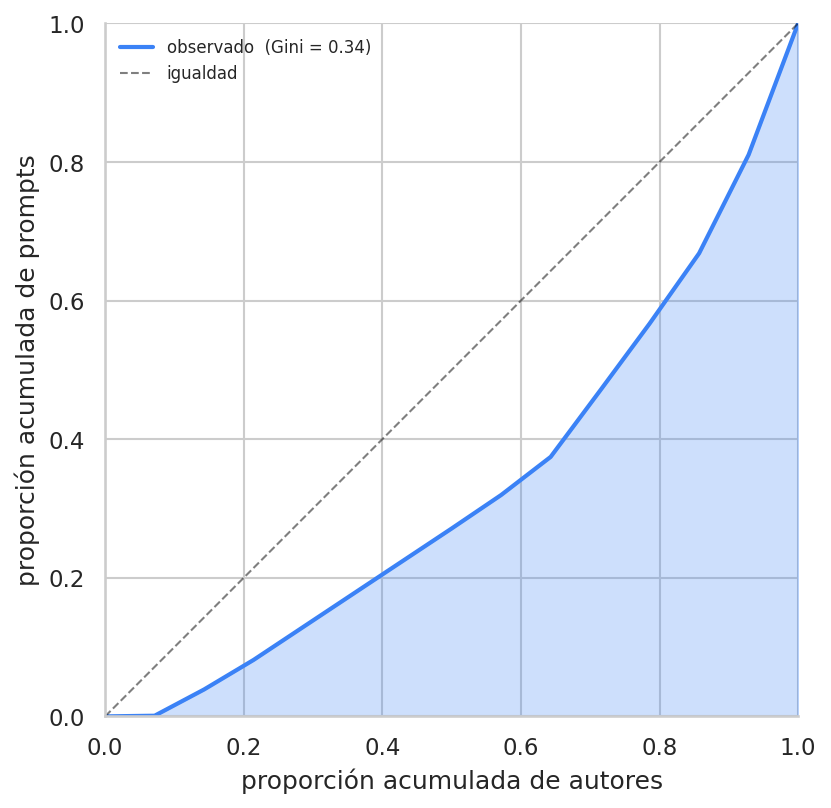
\includegraphics[width=0.95\textwidth]{curva_lorenz.png}
    \caption{Curva de Lorenz de la contribución de prompts por autor. El coeficiente de Gini = $0.34$ (0 = perfecta equidad, 1 = un único autor escribe todo) cuantifica la desigualdad. Métrica importante para citar el dataset: un Gini alto significa que los datos reflejan la idiosincrasia de pocos autores tanto como la del país que dicen representar.}
    \label{fig:curva_lorenz}
\end{figure}
